\begin{abstract}
Terrain rankings can change without identifying a different physical landscape. We compare two scoring contracts at 500 m and 1,000 m support for six Moon and Mars targets using 3,693 overlapping NASADEM windows in the Namib and Atacama. The first contract uses four scaled terrain descriptors; the second combines four descriptor groups with a maximum over 35 sensitivity scenarios. Within a contract, the largest displacement of a winning center is 24.19 km. Between contracts, winners for Jezero and Syrtis move between Namibia and Chile, by 8,349--8,484 km. For Nili Fossae, the scalar top tens share no candidate identifiers, yet their winners are only 3.00 km apart and their 20 km footprints have intersection-over-union 0.739. Five of ten top-ten pairs can be matched one-to-one within 10 km. We release geographic shortlists selected by minimizing the worse rank across supports, with source hashes and reproducible calculations. This post hoc regional result separates identifier turnover, geographic turnover and scoring assumptions. It does not establish a new geological analogue or a safe base location. Independent source-quality and geological checks remain necessary, as illustrated by the accompanying MOLA sampling and lunar pit experiments.
\end{abstract}
\keywords{terrestrial analogues \and NASADEM \and MOLA \and LOLA \and geographic stability}

\section{Research question and contribution}
An Earth location can support a specific exploration task without reproducing an entire lunar or Martian environment. Analogue-site frameworks emphasize selecting for a science or engineering objective rather than an overall impression of fidelity \cite{framework}. MIMESIS addresses regional terrain mapping: comparing relief, slope distributions, terrain organization and surrounding context. It does not estimate rover traction, construction safety or resource abundance.

Adjacent overlapping windows can exchange ranks while retaining much of the same ground. Conversely, two scoring contracts can choose different continents even when each appears stable under a change of support. We test both possibilities using existing Earth--Moon--Mars measurements. The contribution is an original geographic follow-up within this project, with candidate coordinates and explicit limits. We do not claim priority for sensitivity analysis, geographic matching or minimax selection as general methods.

All six targets and both Earth regions were inspected during earlier development. Labels originally called held out no longer confer independent validation. This follow-up is exploratory. Earlier global eligibility, point-support, spectral and feature-scale records use different pools and cannot be combined into a larger apparent sample.

\section{Data and methods}
\subsection{NASA observations and spatial support}
Earth descriptors originate in NASADEM; Mars descriptors use MGS MOLA gridded topography, and lunar descriptors use LRO LOLA \cite{nasadem,mola,lola}. The frozen bundle contains 1,844 Atacama and 1,849 Namib windows. Each local square is 20 km wide, its contextual square is 80 km wide, and candidate centers are separated by 3 km. We compare 500 m and 1,000 m analysis support. Analysis spacing does not imply native source resolution or common information content.

The references are Jezero crater, Nili Fossae, Isidis Planitia and Syrtis Major on Mars, and Taurus--Littrow and the Shackleton rim on the Moon. Descriptors represent fixed study windows, not entire geological provinces. Absolute elevation is excluded from cross-body discrepancy. Both supports must have complete feature vectors. Original products, body-specific coordinates, quality masks and ancestry remain in the source manifests.

\subsection{Two scoring contracts}
The scalar contract uses relief, median slope, upper-decile slope and residual roughness. Relief and roughness use $\log_{10}(x+1)$; slopes remain in degrees. Equal-weight root-mean-square discrepancy uses fixed interquartile scales from the 500 m Earth pool, with standard deviation as fallback. This independently implemented four-variable adaptation retains the provenance of its baseline \cite{terrainfinder}; it differs from that six-variable implementation.

The multigroup contract combines slope-histogram Wasserstein distance, relief and terrain position, roughness and organization, and multiscale context. Weights are 0.40, 0.25, 0.15 and 0.20. Scalar losses use $\min(1,|x-y|/\tau)^2$ with declared engineering tolerances. The score is the maximum over 35 scenarios, including weight perturbations, alternate support and mask erosion. Neither contract has independent geological relevance calibration.

The contracts differ in observables, normalization, weighting and aggregation. This comparison cannot attribute a change to one ingredient. Alternate support already enters the multigroup score; small support shifts there are partly a design consequence, not independent proof of superiority.

\subsection{Geographic comparison and shortlist rule}
Candidates are sorted by score, with ID as the stable tie-breaker. We measure exact top-ten identifier overlap, WGS84 geodesic displacement of winning centers, and square footprint intersection-over-union, $A_{\cap}/A_{\cup}$, in the shared regional azimuthal-equidistant measurement projection. Namibia and Chile are disjoint pools.

Top-ten geographic comparison uses maximum-cardinality one-to-one matching at 5, 10, 20 and 40 km center-distance radii, with total distance breaking ties. A nearby candidate cannot count twice. These radii are exploratory diagnostics relative to the window size, not field-operation tolerances.

For each target and contract, a shortlist entry minimizes the worse full-pool rank across supports. Rank sum and ID break ties, in that order:
\begin{equation}
c^*=\arg\min_c\left(\max\{r_{500}(c),r_{1000}(c)\},\ r_{500}(c)+r_{1000}(c),\ \operatorname{ID}(c)\right).
\end{equation}
This rule avoids choosing a support after seeing its winner. It produces a terrain-screening location, not source qualification or geological validation.

\section{Results}
\subsection{Identifier turnover and shared physical ground}
The scalar contract changes its first-ranked window for four of six targets. Exact top-ten overlaps are 6, 0, 9, 7, 6 and 6 in Figure~\ref{fig:geography}'s order. Winning-center displacements are 24.19, 3.00, 0, 3.00, 0 and 3.00 km. All six scalar winners remain in their respective Earth region when support changes.

For Nili Fossae, no top-ten ID survives, but the winners' footprint intersection-over-union is 73.91\%. Five top-ten pairs match one-to-one within 10 km; seven match within 40 km. Exact turnover therefore exaggerates geographic replacement in this case. It does not establish complete stability: half the top ten cannot be paired within 10 km. The minimax-rank candidate has ranks 17 and 19, outside both top tens.

\begin{figure}[htbp]
\centering
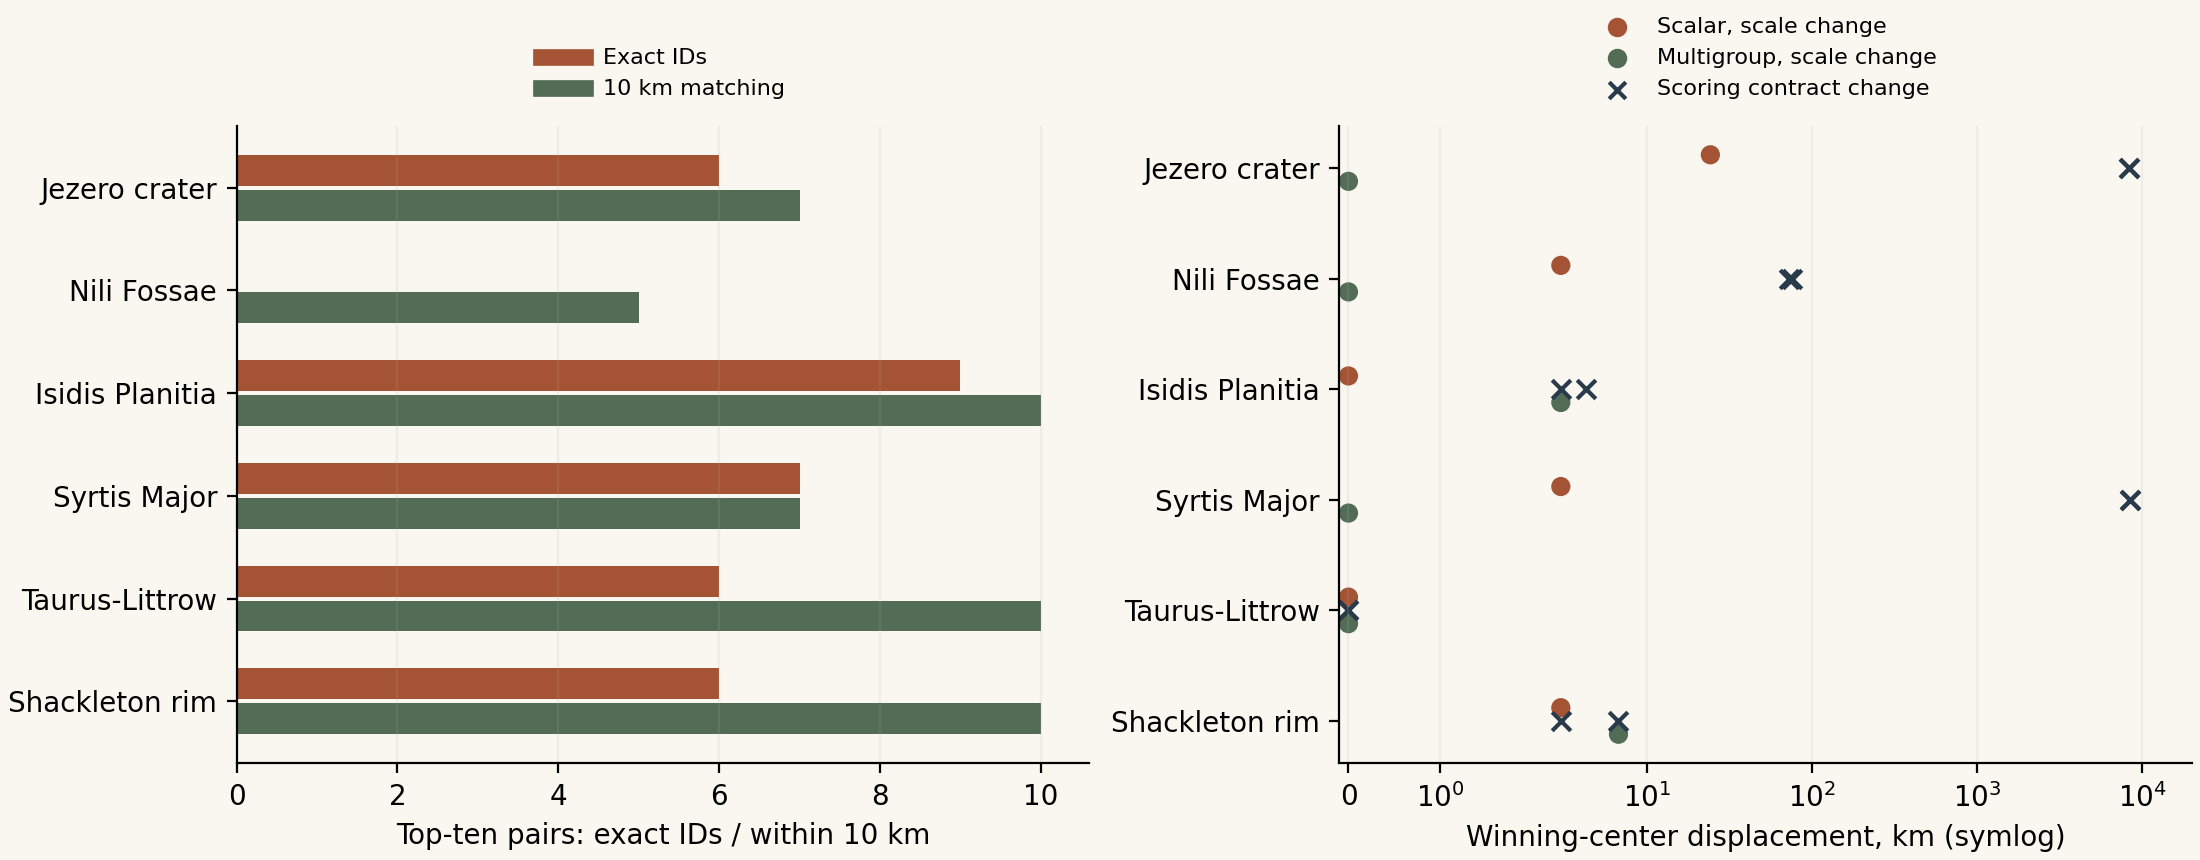
\includegraphics[width=\linewidth]{site-stability.png}
\caption{Left: exact top-ten overlap and maximum one-to-one matches within 10 km for the scalar contract. Right: winning-center displacement under support changes within each contract and contract changes at fixed support. Distance uses a symmetric-logarithmic axis, linear near zero. Conditions are correlated diagnostics, not independent replicates.}
\label{fig:geography}
\end{figure}

\subsection{Scoring assumptions can change the selected continent}
Across twelve within-contract support comparisons, maximum displacement is 24.19 km and median displacement is 1.50 km. Across twelve between-contract comparisons at fixed support, maximum displacement is 8,483.96 km and median displacement is 39.60 km. These are descriptive summaries of inspected conditions, not population estimates or significance tests.

Jezero moves from Namib under the scalar contract to Atacama under the multigroup contract at both supports, by 8,349.27 and 8,360.17 km. Syrtis moves in the opposite direction by 8,482.86 and 8,483.96 km. Nili stays in Namib but moves 72.50--75.24 km between contracts. Isidis differs by 3.00--4.24 km; Taurus--Littrow agrees exactly; Shackleton differs by 3.00--6.71 km.

For these contracts and this pool, agreement across two supports does not imply agreement across scoring assumptions. Choosing a contract after seeing a preferred region would hide a consequential decision. No observed geological or operational outcome establishes that either contract is better.

\subsection{Earth locations for follow-up}
Table~\ref{tab:shortlist} provides scalar minimax-rank coordinates. The GeoJSON includes twelve target--contract entries with footprints, ranks and source IDs. Repeated windows are retained as target relationships, not counted as independent sites. Both contracts select the same minimax window for Taurus--Littrow and the same minimax window for Shackleton.

\begin{table}[htbp]
\centering\small
\caption{Exploratory scalar shortlist. WGS84 window centers are not surveyed features or field destinations. Ranks correspond to 500 m and 1,000 m support. N = Namib; A = Atacama.}
\label{tab:shortlist}
\begin{tabular}{llrrl}
\toprule
Target & Pool & Latitude & Longitude & Ranks\\
\midrule
Jezero & N & -25.35098 & 15.43375 & 1 / 4\\
Nili Fossae & N & -25.16248 & 16.05951 & 17 / 19\\
Isidis & N & -24.61966 & 16.59254 & 1 / 1\\
Syrtis & A & -23.45714 & -68.41277 & 1 / 2\\
Taurus--Littrow & A & -24.43210 & -68.37876 & 1 / 1\\
Shackleton & A & -24.43233 & -68.43792 & 3 / 1\\
\bottomrule
\end{tabular}
\end{table}

These coordinates support a follow-up desk study of terrain mapping. They do not establish previously unrecognized geological analogues: both regional pools are established analogue environments, and local process relevance has not been validated here. A terrain match alone does not reproduce the lunar or Martian atmosphere, gravity, radiation, thermal regime, polar illumination or mineralogy.

\section{Source checks and independent evidence}
A separate diagnostic transfers six actual MOLA point patterns to three Earth fields. ODE distinguishes PEDR point observations from gridded MEGDR products \cite{ode}. Of 103,371 returned points, 102,240 survive the retained spatial and attitude rules. Bilinear sampling precedes linear reconstruction at 500 m, with no extrapolation and a 1,000 m observation-distance cutoff. All eighteen comparisons lower median slope on their common masks; RMSE spans 14.33--28.65 m and common derivative-valid coverage spans 35.5--56.4\%. Appendix~\ref{app:support} retains every outcome.

Geometry and reconstruction change together in that experiment. It neither reproduces original MEGDR interpolation nor isolates a causal geometry effect. Original shot-quality fields and unique identities are absent. CTX DTMs aligned to MOLA are not fully independent elevation references \cite{ctx}. Descriptor agreement therefore cannot certify planetary terrain accuracy.

The separate global eligibility record has zero qualified contexts out of 100, with eighteen terrain exclusions, 49 observed natural-land upper-bound exclusions and 33 unknown outcomes. Those counts do not describe the regional ranking pool. Missing layers do not establish unsuitable terrain. Earlier eligible Namib pools also contain no independent context-separated control pair; Appendix~\ref{app:gates} explains the geometric limitation.

USGS SIM 3464 provides Jezero calibration geology \cite{jezero}, while the prospective Mars windows lack corresponding independent reference zones. Five of eleven EMIT masks contain eligible native centers; one has reflectance-and-uncertainty analysis \cite{emit}. The inspected CRISM example lacks its reflectance cube and assigned geological labels. Known Puga laboratory samples cannot substitute for registered orbital geology. No mineral-validation outcome is claimed.

The lunar pit pilot also stops before nomination. Successful-correlation coverage of 93.42\% at Tranquillitatis and 97.37\% at Marius Hills falls to usable exterior coverage of 0\% and 1.56\% after the 10 m Gaussian neighborhood mask. Both have zero at 20 and 40 m, against a 95\% requirement. All 120 source-mask sensitivities fail, despite successful analytical-plane controls. Appendices~\ref{app:pilot} and \ref{app:protocol} preserve the source ledger and stopping rule. A revised local-plane estimator has promising numerical controls, not completed geological calibration.

\section{Use, limitations and novelty boundary}
A mapping team could use the shortlist to compare terrain organization and decide which observations to acquire next. That is an intended use, not a measured saving in mission cost or improvement in training. Source eligibility, local geology, access and independent task performance remain unresolved. More downloads cannot substitute for process-relevant reference observations or human-task outcomes.

The pool contains two regions, squares overlap strongly, targets were already inspected, and matching radii are post hoc diagnostics. We do not bootstrap overlapping windows as independent sites. The report retains both contracts and all six cases, including weak cross-support compromise. World-first priority is not established; prior analogue and morphometric work constrains broad originality claims \cite{roughness,jingpo,asymmetry,cotm,framework}.

The new project finding is the measured separation between ID turnover, shared ground and contract-driven location changes. A new geological analogue would additionally require a distinct candidate area, process evidence, comparison with known sites and independent validation. The unfinished confirmatory feature-scale study remains unfinished.

\section{Reproducibility and disclosure}
Run \path{python scripts/measure_site_stability.py} from the repository root to regenerate the geographic JSON, GeoJSON, figures and application record from the shipped bundle. The output records its SHA-256 and implementation hashes. This reproduces descriptor-level calculations, not raw elevation acquisition. Earlier source ancestry remains in the bundle manifests; source-dependent reconstruction uses separate workflows.

Explore preserves the ranking workspace. Evidence opens the geographic finding and retains the calibration and source diagnostics. Methods and Data expose contracts and exports. The paper, source archive and submission brief are included in the public repository. Restricted cave surveys and unresolved redistribution inputs are excluded. Appendix~\ref{app:claims} distinguishes the attributed baseline replication from the new geographic follow-up.

Arjun Vijay Prakash built the project as a Grade XI student at City Montessori School, Kanpur Road, Lucknow, India. Codex assisted with implementation, analysis code and writing. No independent expert review, field validation, peer review or NASA endorsement is claimed. The supplied Overleaf template uses the \texttt{arxiv} style \cite{template}; it does not imply arXiv deposition.
